% !TeX root = ../../main.tex
\section{Hydraulic wash column design}

Commonly used solid-liquid separators are not continuous processes, typically batch or semi-batch. Wash column does wash and continuous transport in one process. Whereas, for example a centrifuge would require  melting the crystals and a means of solid transport by conveyor belt. Different type of wash columns include gravity, hydraulic and mechanical. Hydraulic was chosen because of shorter residence time and less moving mechanical parts. 

\subsection{Steady State Model}   

Typically, the design of a hydraulic wash column will be based on pilot-scale experiments to determine appropriate dimensions at varying operating conditions. Instead, a  model from literature \cite{van_oord-knol_hydraulic_2000} was used to estimate the performance of the column at steady state. The hydraulic wash column was modelled based on volume and force balance using initial dimensions \cite{oordknol_dynamic_2002}. The initial dimensions were varied to determine the performance of the column handling the output from the MSMPR crystalliser. The aim of this model was to determine an appropriate steer flow rate, feasible column diameter and determine the pressure at different sections of the wash column.

\begin{wrapfigure}{L}{0.5\linewidth}
\centering
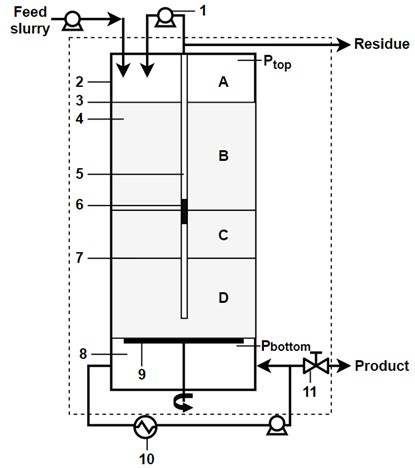
\includegraphics[width=0.5\textwidth]{figures/hydraulic.jpg}
\caption{A schematic diagram of the hydraulic wash column:1) steer flow pump 2) column wall 3)bed level 4) packed bed 5) filter tube 6) filter 7) wash front level 8) reslurry section 9) knife 10) melter 11) product flow valve; A) slurry section B) filtration section C) stagnant sectino D) wash front section \cite{van_oord-knol_hydraulic_2000}}
\label{fig:hydraulic}
\end{wrapfigure}

Purification in the hydraulic column occurs through displacement and crystallisation of wash liquid on the crystals. This model assumes 100 \% solid-liquid separation in the wash column therefore no presence of liquid in the product flow rate as the pressure difference is large enough to ensure no mother liquor enters the wash front. TNO had developed the TNO HWC which provides chemicals with purity greater than 99.9\% (TNO melt crystallisation). However, if impurities are entrapped in the crystal lattice during crystallisation, these will not be removed. This highlights the disadvantage of hydraulic wash column compared to gravity wash column. Gravity wash column allows some impurities to be removed from the crystals during the long residence time. 

Figure \ref{fig:hydraulic} illustrates the different components in the hydraulic column. The different sections in the column are characteristic of the column. The feed slurry contains a mixture of m-nitrotoluene (mother liquor) and p-nitrotoluene (solid crystals) from the MSMPR crystalliser. This enters the column in slurry section. Due to difference in density the solid crystals will begin to fall down the column. As the crystals move down the column it forms a packed bed of solid. The filter in the filter tube removes the mother liquor from the filtration section. A part of the mother liquor gets recycled back into the column by the steer pump, known as steer flow and some mother liquor is purged out as residue flow. The pressure drop across the filter drives the solids down and the mother liquor up the filter tube allowing for solid-liquid separation. The solid deposits as densely packed moving bed in the wash front section with no mother liquor present. The knife at the bottom will cut the bottom of the packed bed so pure p-nitrotoluene solids will fall into the bottom section. The melter at the bottom melts the p-nitrotoluene solids and forms what is known as the washing liquid. The washing liquid gets recycled around the bottom section. Due to the pressure drop at the valve when the product gets purged out, the washing liquid gets pushed up into the washing section of the column where counter current washing occurs. The solid crystals are of a lower temperature and causes the washing liquid to crystallise on the solid particles leading to a frozen wash front level. This counter current washing allows for almost 100 \% separation. 

\subsubsection{Volume balance} 
This model was based on the assumption that the liquid and solid in the system were incompressible. For simplicity density and viscosity were assumed to be independent of temperature. 

Overall volume balance at the top section 
\begin{equation}
\phi_{\mathrm{feed}}+\phi_{\mathrm{steer}}=\phi_{s,\mathrm{filters}}+\phi_{ml.\mathrm{filters}}
\end{equation}

The total length of the top section is constant. The length of the filtration section was derived from the solid balance in the top section. 

\begin{equation}
\frac{dL_{\mathrm{filtration}}}{dt} = \frac{1}{A_c(1-\alpha_2-\epsilon)}(\alpha_1\phi_{\mathrm{feed}}-\phi_{s,\mathrm{filters}})
\end{equation}

In the bottom section, there is the stagnant zone with the crystals. Then there is the wash zone with only the crystal and the wash liquid at steady state. The wash liquid crystallises due to the low temperature at the wash front. The crystallisation of the wash liquid can be related to the disappearance of the wash liquid by difference in density of the solid and liquid.

\begin{equation}
C_l= \frac{\rho_s}{\rho_l}C_s
\end{equation}

The amount of crystallised material was calculated based on a heat balance and temperature difference between the feed and the melt. This assumes the total cooling capacity of the crystals is used to crystallise the wash liquid. 

\begin{equation}
C_s= \frac{c_p(T_{\mathrm{melt}}-T_{\mathrm{feed}})}{\Delta H_m}Q_{s,\mathrm{filters}}
\end{equation}

The length of the wash section is related to the wash-liquid flow entering the knife and the wash liquid that crystallises. This assumes the wash liquid is not loss through the filters which is ensured by positioning the filters above the wash section.

\begin{equation}
\epsilon_w A_c \frac{dL_{\mathrm{wash}}}{dt}= \phi_{wl,\mathrm{knife}}-C_l
\end{equation}

The wash column during operation forms 3 layers of filtration, stagnant and wash sections. Within the filtration and stagnant section it is assumed the porosity and permeability remain constant. Since the crystals form a densely packed column $\epsilon$ was taken as 0.45. Due to the wash-liquid crystallisation at the wash zone an abrupt change in porosity and permeability was considered. The consolidation of the crystal bed were neglected in this model, however under compressive force from the pressure at the top section this may not be a valid assumption and will have to be further evaluated in a pilot scale experiment. The porosity in the wash zone was calculated from the equation below. 

\begin{equation}
\epsilon_{w}= \epsilon-(1-\epsilon)\left(\frac{c_p(T_{\mathrm{melt}}-T_{\mathrm{feed}})}{\Delta H_m}\right)
\end{equation}

At steady state, the wash section is constant therefore there  would be no flow of mother liquor into or out of the bottom section. The mother liquor at the top section leaves the column through the filter and splits into residual and steer flow. 

\begin{equation}
\phi_{\mathrm{residue}}= \phi_{ml,\mathrm{filters}} - \phi_{\mathrm{steer}}
\end{equation}

The volume balance at the melting circuit is based on the assumption that crystals are molten the moment they enter the melting circuit. The wash liquid enters the column at the melting temperature. 

\begin{equation}
\frac{\rho_s}{\rho_l}\phi_{s,\mathrm{knife}}= \phi_{wl,\mathrm{knife}} - \phi_{\mathrm{product}}
\end{equation}


\subsubsection{Force balance}
The liquid pressure drop across each section were calculated with the following modified Darcy's law equation. 

\begin{equation}
\frac{\Delta P_{l,\mathrm{filtration}}}{L_{\mathrm{filtration}}}=\frac{\epsilon \eta_{l}}{B_{\mathrm{filtration}}}\left(\frac{\phi_{ml,\mathrm{filters}}}{\epsilon A_c} - \frac{\phi_{s,\mathrm{filters}}}{1-\epsilon A_c}\right)
\end{equation}

\begin{equation}
\frac{\Delta P_{l,\mathrm{stagnant}}}{L_{\mathrm{stagnant}}}=\frac{\epsilon \eta_{l}}{B_{\mathrm{stagnant}}}\left(-\frac{\phi_{ml,\mathrm{bottom}}}{\epsilon A_c} - \frac{\phi_{s,\mathrm{filters}}}{1-\epsilon A_c}\right)
\end{equation}

\begin{equation}
\frac{\Delta P_{l,\mathrm{wash}}}{L_{\mathrm{wash}}}=\frac{\epsilon \eta_{l}}{B_{\mathrm{wash}}}\left(-\frac{\phi_{wl,\mathrm{knife}}}{\epsilon_w A_c} - \frac{\phi_{s,\mathrm{knife}}}{1-\epsilon_w A_c}\right)
\end{equation}

The liquid pressure gradient at each section were assumed to be constant due to the incompressibilty assumption of the packed bed. The liquid pressure at the top in the slurry section was based on the pressure at the filter and the pressure drop over the filtration section. 

\begin{equation}
P_{\mathrm{top}} = P_{\mathrm{filters}} + \Delta P_{l,\mathrm{filtration}}
\end{equation}


The pressure at the bottom is equal to the pressure drop in the valve of the melting circuit. This pressure drop across the valve is determined through a linear relation with the product flow rate.

\begin{equation}
P_{\mathrm{bottom}}=\Delta P_{\mathrm{valve}} = K_w\phi_{\mathrm{product}}
\end{equation}

%The pressure after the valve is atmospheric.
The pressure in the melting circuit was calculated using the equation below. 

\begin{equation}
\Delta P_{\mathrm{valve}} = \Delta P_{l,\mathrm{stagnant}} + \Delta P_{l,\mathrm{wash}} + P_{\mathrm{filters}}
\end{equation}


\subsection{Results and Discussion}
The linear system of equations from the steady state model were solved using input variables and parameters shown in Table \ref{tab:inputsparameters}. 

\begin{table}[h]
\centering
\caption{Input variables and parameters}
\label{tab:inputsparameters}
\begin{tabular}{lS[table=format=1.3e2]s|lS[table=format=1.2e+2]s}
\toprule
\multicolumn{3}{c|}{\textbf{Inputs}}                     & \multicolumn{3}{c}{\textbf{Parameters}}          \\ \midrule
$\phi_{\mathrm{feed}}$  & 4.27e5 & \cubic\m\per\s        & $\epsilon$                & 0.45     &           \\
$\phi_{\mathrm{steer}}$ & 2.65e5 & \cubic\m\per\s        & $\mathrm{B_{filtration}}$ & 1.37e-13 & \square\m \\
$\alpha_1$              & 0.906  & v/v                   & $\mathrm{B_{wash}}$       & 1.01e-13 & \square\m \\
$\mathrm{K_{w}}$        & 1.9e10 & \pascal\s\per\cubic\m &                           &          &           \\ \bottomrule
\end{tabular}
\end{table}

During operation of the hydraulic column  variations in the length of the filtration, stagnant and wash section is possible. Therefore, simulations of variable filtration and wash section lengths were implemented on Excel to determine the effect on pressures at different sections of the column. With proper controls in place, the sections should not vary significantly during normal operation, therefore variation in filtration and wash section would be designed to be between 0.27 to 0.30 m.  

\begin{wrapfigure}{L}{0.5\linewidth}
\centering
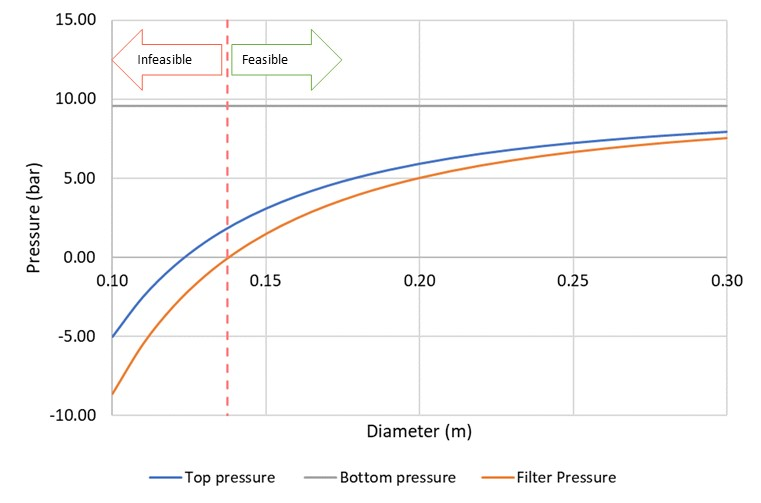
\includegraphics[width=0.5\textwidth]{chapters/3-separation/figures/diameter.jpg}
\caption{ Effect of varying diameter}
\label{fig:dia_col}
\end{wrapfigure}

The length of the column was fixed at 0.8 m. The diameter of the column was varied from 0.1 m to 0.3 m to observe the impact it has on the pressure across the column. Figure \ref{fig:dia_col} indicates below 0.165 m the model suggests negative pressure at the filter which could imply instead of mother liquor flowing up through the filter tube, it could be flowing in the reverse direction. The pressure at the top is also negative indicating at these conditions the fluid flow in the column may not be in the desirable downward direction. A suitable diameter was chosen at 0.17 m allowing for slight variations in the section lengths over time under normal operation.

\begin{wrapfigure}{L}{0.5\linewidth}
\centering
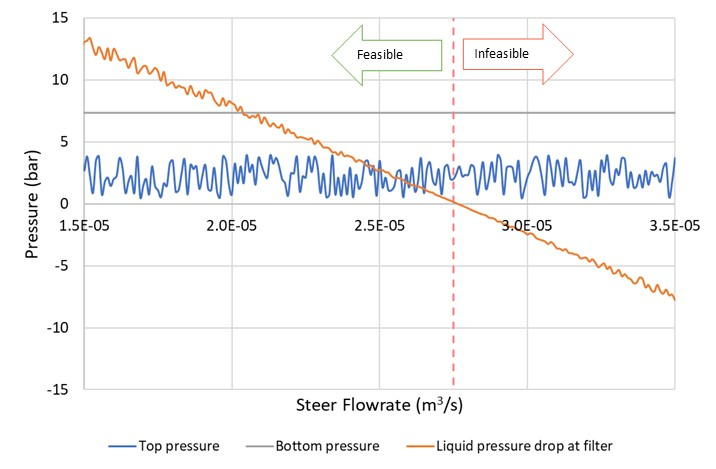
\includegraphics[width=0.5\textwidth]{chapters/3-separation/figures/steerflow.jpg}
\caption{ Effect of varying steer flow rate}
\label{fig:steer_col}
\end{wrapfigure}

Steer flow is the flow rate of the mother liquor being recycled back into the column from the filter tubes whilst some mother liquor are removed as residual flow. The filtrate being recycled back into the column increases the transport force. Steer flowrate was varied from 1.5e-5 to 3.5e-5 m3/s. Figure \ref{fig:steer_col} shows the unfeasible and feasible region of operation. Above a steer flow 2.7e-5, the column starts exhibiting negative liquid pressure drop at the filter. However, at lower steer flow such as 1.5e-5 the filter pressure increases significantly to more than 10 bar. In order to attain a lower pressure but also ensure the column is in a feasible region, the steer flow at 2.65 e-5 was chosen. At this flow rate there is an allowance for variation in the flowrate whilst the column is still operating in the feasible region. The steer flow has no impact on the bottom pressure and the top pressure. This is because the bottom pressure relies on the valve resistance coefficient. 

\begin{wrapfigure}{L}{0.5\linewidth}
\centering
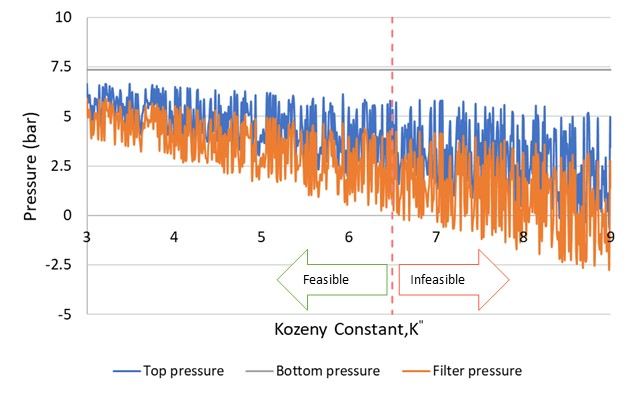
\includegraphics[width=0.5\textwidth]{chapters/3-separation/figures/kozeny.jpg}
\caption{ Effect of varying Kozeny constant}
\label{fig:koz_col}
\end{wrapfigure}

A sensitivity analysis on the permeability constant was conducted by varying the Kozeny constant, K". 

Based on literature \cite{jansens_furification_1995}, the temperature profile at the wash front was found to be independent of the axial and radial position in the column if the distance of the wash front from the filter is greater than 0.1 m. In this design the filter tube was positioned 0.1 m above the wash front. The temperature profile was also found to be independent of the product throughput.  


\subsection{Materials Choice}
- material for the column itself 

\subsection{Mechanical Design}
-BS standard has to be followed since column maximum operating pressure is 9.8 bar. It is a pressure vessel.  
